% ==============================================================================
% Lecture 1: Introduction to Marketing Research
% MKTG5012 Marketing Research — CUHK Business School
% ==============================================================================

% ==============================================================================
% Beamer Preamble: MKTG5012 Marketing Research — CUHK
% ==============================================================================

% --- Document class ---
\documentclass[aspectratio=169, 11pt]{beamer}

% --- Theme ---
\usetheme{Madrid}
\usecolortheme{default}

% --- CUHK Institutional Colors ---
\definecolor{cuhkpurple}{HTML}{6B2D8B}
\definecolor{cuhkgold}{HTML}{EDAB56}
\definecolor{darkgray}{HTML}{3D3D3D}
\definecolor{positive}{HTML}{15803d}
\definecolor{negative}{HTML}{b91c1c}
\definecolor{lightbg}{HTML}{F5F0FA}

% --- Apply CUHK colors to theme ---
\setbeamercolor{structure}{fg=cuhkpurple}
\setbeamercolor{palette primary}{bg=cuhkpurple, fg=white}
\setbeamercolor{palette secondary}{bg=cuhkgold, fg=darkgray}
\setbeamercolor{palette tertiary}{bg=darkgray, fg=white}
\setbeamercolor{frametitle}{bg=cuhkpurple, fg=white}
\setbeamercolor{title}{fg=white, bg=cuhkpurple}
\setbeamercolor{subtitle}{fg=cuhkgold}
\setbeamercolor{block title}{bg=cuhkpurple, fg=white}
\setbeamercolor{block body}{bg=lightbg, fg=darkgray}
\setbeamercolor{block title alerted}{bg=negative, fg=white}
\setbeamercolor{block body alerted}{bg=negative!10, fg=darkgray}
\setbeamercolor{block title example}{bg=positive, fg=white}
\setbeamercolor{block body example}{bg=positive!10, fg=darkgray}
\setbeamercolor{item}{fg=cuhkpurple}
\setbeamercolor{footline}{fg=darkgray}

% --- Fonts ---
\usepackage{fontspec}
\setsansfont{Helvetica Neue}[
  BoldFont = {Helvetica Neue Bold},
  ItalicFont = {Helvetica Neue Italic}
]
\setmonofont{Menlo}[Scale=0.85]

% --- Packages ---
\usepackage{graphicx}
\usepackage{booktabs}
\usepackage{colortbl}
\usepackage{amsmath, amssymb}
\usepackage{tikz}
\usetikzlibrary{shapes, arrows.meta, positioning, fit, calc}
\usepackage{hyperref}
\usepackage{xeCJK}
\setCJKmainfont{PingFang SC}

% --- Bibliography ---
\usepackage[style=authoryear, backend=biber, maxcitenames=2]{biblatex}
\addbibresource{Bibliography_base.bib}

% --- Footer ---
\setbeamertemplate{navigation symbols}{}
\setbeamertemplate{footline}{%
  \leavevmode%
  \hbox{%
    \begin{beamercolorbox}[wd=.33\paperwidth,ht=2.5ex,dp=1ex,left]{footline}%
      \hspace*{2ex}\footnotesize MKTG5012 Marketing Research
    \end{beamercolorbox}%
    \begin{beamercolorbox}[wd=.34\paperwidth,ht=2.5ex,dp=1ex,center]{footline}%
      \footnotesize CUHK Business School
    \end{beamercolorbox}%
    \begin{beamercolorbox}[wd=.33\paperwidth,ht=2.5ex,dp=1ex,right]{footline}%
      \footnotesize \insertframenumber/\inserttotalframenumber\hspace*{2ex}
    \end{beamercolorbox}%
  }%
  \vskip0pt%
}

% --- Custom commands ---
\newcommand{\cmark}{\textcolor{positive}{\checkmark}}
\newcommand{\xmark}{\textcolor{negative}{$\times$}}
\newcommand{\source}[1]{\vfill\hfill{\scriptsize\textcolor{gray}{#1}}}
\newcommand{\rcode}[1]{\texttt{\textcolor{cuhkpurple}{#1}}}
\newcommand{\highlight}[1]{\textcolor{cuhkpurple}{\textbf{#1}}}

% --- Code listing style ---
\usepackage{listings}
\lstset{
  language=R,
  basicstyle=\ttfamily\small,
  keywordstyle=\color{cuhkpurple}\bfseries,
  stringstyle=\color{positive},
  commentstyle=\color{gray}\itshape,
  numbers=none,
  frame=single,
  rulecolor=\color{cuhkpurple!30},
  backgroundcolor=\color{lightbg},
  breaklines=true,
  showstringspaces=false,
  columns=fullflexible,
  literate={<-}{{$\leftarrow$}}2
}


\title{Lecture 1: Introduction to Marketing Research}
\subtitle{Defining the Problem and Developing an Approach}
\author{Jasmine Yang}
\institute{CUHK Business School}
\date{MKTG5012 --- Term 1, 2025--26}

\begin{document}

% ======================================================================
% ACT 0: COURSE WELCOME & LOGISTICS
% ======================================================================

\begin{frame}
  \titlepage
\end{frame}

% ------------------------------------------------------------------
\begin{frame}{About Your Instructor}
  \begin{columns}
    \begin{column}{0.65\textwidth}
      \textbf{Jasmine Yang}

      \vspace{1em}
      \begin{itemize}
        \item Instructor, MKTG5012 Marketing Research
        \item CUHK Business School
      \end{itemize}

      \vspace{1em}
      \textbf{Contact}
      \begin{itemize}
        \item Office hours: By appointment
        \item Email: See Blackboard
      \end{itemize}
    \end{column}
    \begin{column}{0.3\textwidth}
      % Placeholder for instructor photo
      
\begin{tikzpicture}
        \draw[cuhkpurple, thick, rounded corners]
          (0,0) rectangle (3,3.5);
        \node[text=gray] at (1.5,1.75) {Photo};
      \end{tikzpicture}
    \end{column}
  \end{columns}
\end{frame}

% ------------------------------------------------------------------
\begin{frame}{Course Overview}
  \begin{block}{Two Key Learning Goals}
    \begin{enumerate}
      \item \textbf{Marketing theory:} Apply marketing concepts, principles,
            and theories to implement effective marketing operations
      \item \textbf{Analytical techniques:} Apply advanced analytical and
            quantitative techniques to make sound marketing decisions
    \end{enumerate}
  \end{block}

  \vspace{1em}
  On completion, you will be able to:
  \begin{itemize}
    \item Understand key stages of the research process
    \item Work with data to produce quantitative and qualitative evidence
    \item Think strategically about \emph{whether} and \emph{how} to do
          marketing research
    \item Communicate findings persuasively
  \end{itemize}
\end{frame}

% ------------------------------------------------------------------
\begin{frame}{Assessment}
  \begin{columns}
    \begin{column}{0.48\textwidth}
      \begin{block}{Group Assessment (55\%)}
        \begin{tabular}{lr}
          \toprule
          Component & Weight \\
          \midrule
          Product concepts & 10\% \\
          Questionnaire & 10\% \\
          Research report & 15\% \\
          Presentation & 20\% \\
          \bottomrule
        \end{tabular}
      \end{block}
    \end{column}
    \begin{column}{0.48\textwidth}
      \begin{block}{Individual Assessment (45\%)}
        \begin{tabular}{lr}
          \toprule
          Component & Weight \\
          \midrule
          Class participation & 15\% \\
          Examination & 30\% \\
          \bottomrule
        \end{tabular}
      \end{block}
      \vspace{0.5em}
      {\small Groups of up to 8 students.\\
      Form groups by Week 3.}
    \end{column}
  \end{columns}
\end{frame}

% ------------------------------------------------------------------
\begin{frame}{AI Tools Policy}
  \begin{alertblock}{Approach 2: Use with Acknowledgment}
    AI tools (ChatGPT, Gemini, etc.) may be used for assignments and group
    projects \textbf{with prior permission and proper acknowledgment}.
  \end{alertblock}

  \vspace{0.5em}
  \begin{itemize}
    \item \textcolor{positive}{\textbf{Allowed:}} Enhance understanding,
          improve writing, explore analytical processes
    \item \textcolor{negative}{\textbf{Not allowed:}} Generate drafts or
          solutions directly; use in \textbf{final exam}
    \item Ideas and drafts should be the student's \textbf{original work}
  \end{itemize}

  \vspace{0.5em}
  \begin{exampleblock}{Key Principle}
    AI tools could enhance our learning outcome, but never replace our
    efforts to learn. \emph{Learn with and from AI; learn to think without AI.}
  \end{exampleblock}
\end{frame}

% ------------------------------------------------------------------
\begin{frame}{Course Schedule}
  {\scriptsize
  \begin{tabular}{clll}
    \toprule
    \textbf{\#} & \textbf{Topic} & \textbf{R Lab} & \textbf{Reading} \\
    \midrule
    \rowcolor{cuhkpurple!10}
    1 & Intro to MR; Problem Definition & Install, Console, RStudio
      & M 1--2; L 1--2 \\
    2 & Product Development & Arithmetic, Functions, Library
      & Iansiti; L 3 \\
    3 & Concept Test; Research Design & Conditions, Loop
      & Fernbach; M 3 \\
    4 & Exploratory Research Design & Read/Write Files
      & M 4--6 \\
    5 & Descriptive Research; Scaling & ---
      & M 6, 8 \\
    6 & Scaling; Questionnaire Design & $\chi^2$, $r$, $t$-test
      & M 9--10; L 4--5 \\
    7 & Hypothesis Testing; ANOVA & ANOVA
      & M 15--16; L 6 \\
    8 & Regression; Sampling & Regression
      & M 17, 11--12; L 7--8 \\
    9 & Fieldwork; Data Prep; Reporting & NLP, Web Scraping
      & M 13--14, 23 \\
    10 & Experimentation; Market Sizing & Graphics
       & M 7 \\
    \bottomrule
  \end{tabular}
  }

  \vspace{0.3em}
  {\footnotesize M = Malhotra (2020); L = Lam (2023)}
\end{frame}

% ======================================================================
% ACT 1: WHAT IS MARKETING?
% ======================================================================

\begin{frame}{}
  \begin{center}
    {\Large\textcolor{cuhkpurple}{\textbf{Part I}}}\\[0.5em]
    {\LARGE\textbf{What is Marketing?}}\\[1em]
    {\normalsize Lam (2023), Chapter 1}
  \end{center}
\end{frame}

% ------------------------------------------------------------------
\begin{frame}{Do You Check Reviews Before Buying?}
  \begin{center}
    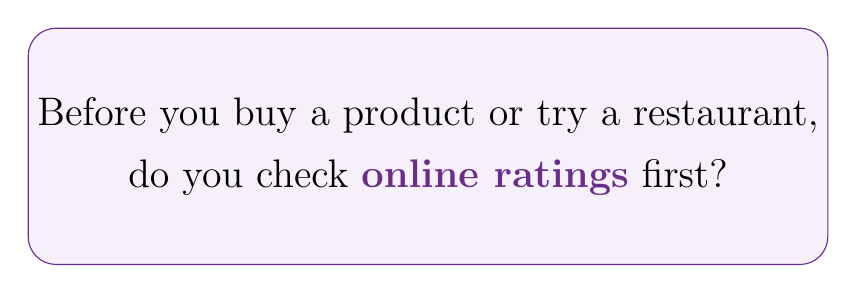
\begin{tikzpicture}
      \node[draw=cuhkpurple, fill=lightbg, rounded corners=10pt,
            minimum width=10cm, minimum height=3cm, align=center,
            font=\Large] {
        Before you buy a product or try a restaurant,\\[0.3em]
        do you check \textcolor{cuhkpurple}{\textbf{online ratings}} first?
      };
    \end{tikzpicture}
  \end{center}

  \vspace{1em}
  Think about:
  \begin{itemize}
    \item \emph{What information} are you looking for?
    \item \emph{Where} do you find it?
    \item \emph{How} does it influence your decision?
  \end{itemize}

  \vspace{0.5em}
  \textcolor{cuhkpurple}{$\rightarrow$ You are already doing a form of
    ``marketing research''!}
\end{frame}

% ------------------------------------------------------------------
\begin{frame}{Marketing as Exchange}
  \begin{columns}
    \begin{column}{0.45\textwidth}
      \begin{block}{AMA Definition}
        ``Marketing is the activity, set of institutions, and processes for
        \textbf{creating, communicating, delivering, and exchanging} offerings
        that have value for customers, clients, partners, and society at
        large.''
      \end{block}
      \source{AMA (2023); Lam (2023), p.1}
    \end{column}
    \begin{column}{0.5\textwidth}
      % Exchange triangle diagram (Lam Fig 1.1)
      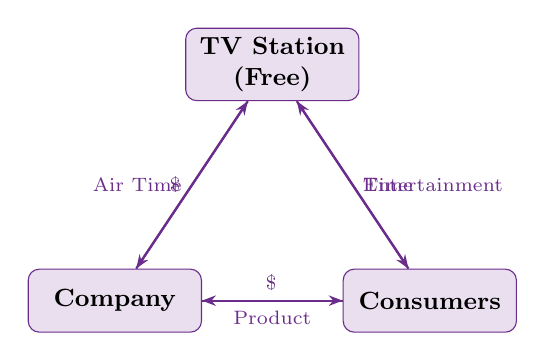
\begin{tikzpicture}[
        node distance=2.5cm,
        box/.style={draw=cuhkpurple, fill=cuhkpurple!15, rounded corners,
                     minimum width=2.2cm, minimum height=0.8cm,
                     font=\small\bfseries, align=center},
        arr/.style={-{Stealth[length=5pt]}, thick, cuhkpurple}
      ]
        \node[box] (tv) at (2,3.5) {TV Station\\(Free)};
        \node[box] (co) at (0,0.5) {Company};
        \node[box] (cu) at (4,0.5) {Consumers};

        \draw[arr] (co) -- node[left, font=\scriptsize] {\$} (tv);
        \draw[arr] (tv) -- node[left, font=\scriptsize] {Air Time} (co);
        \draw[arr] (tv) -- node[right, font=\scriptsize] {Entertainment} (cu);
        \draw[arr] (cu) -- node[right, font=\scriptsize] {Time} (tv);
        \draw[arr] (co) -- node[below, font=\scriptsize] {Product} (cu);
        \draw[arr] (cu) -- node[above, font=\scriptsize] {\$} (co);
      \end{tikzpicture}
    \end{column}
  \end{columns}
\end{frame}

% ------------------------------------------------------------------
\begin{frame}{The 5Cs (+ Consumer) Framework}
  \begin{center}
    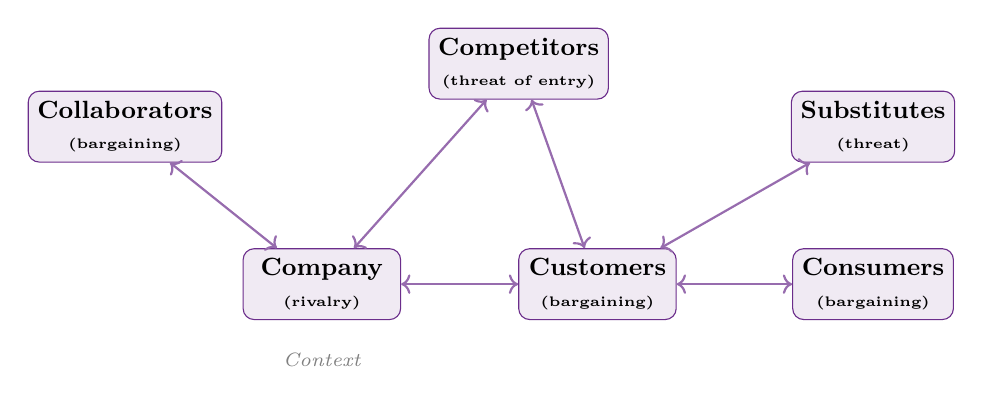
\begin{tikzpicture}[
      box/.style={draw=cuhkpurple, fill=cuhkpurple!10, rounded corners,
                   minimum width=2cm, minimum height=0.9cm,
                   font=\small\bfseries, align=center},
      arr/.style={-{Stealth[length=4pt]}, thick, cuhkpurple!70}
    ]
      \node[box] (comp) at (0,0) {Company\\{\tiny(rivalry)}};
      \node[box] (cust) at (3.5,0) {Customers\\{\tiny(bargaining)}};
      \node[box] (cons) at (7,0) {Consumers\\{\tiny(bargaining)}};
      \node[box] (coll) at (-2.5,2) {Collaborators\\{\tiny(bargaining)}};
      \node[box] (cmpt) at (2.5,2.8) {Competitors\\{\tiny(threat of entry)}};
      \node[box] (subs) at (7,2) {Substitutes\\{\tiny(threat)}};
      \node[below=0.3cm of comp, font=\scriptsize\itshape, text=gray]
        {Context};

      \draw[arr, <->] (comp) -- (cust);
      \draw[arr, <->] (cust) -- (cons);
      \draw[arr, <->] (comp) -- (coll);
      \draw[arr, <->] (comp) -- (cmpt);
      \draw[arr, <->] (cust) -- (cmpt);
      \draw[arr, <->] (cust) -- (subs);
    \end{tikzpicture}
  \end{center}

  \vspace{0.3em}
  {\small
  \textbf{Customers} buy from the company (e.g., retailers).
  \textbf{Consumers} use the product.
  The \textbf{Context} includes culture, regulations, and environmental factors.}
  \source{Dolan (2019); Porter (2008); Lam (2023), pp.2--3}
\end{frame}

% ------------------------------------------------------------------
\begin{frame}{Segmentation, Targeting, Positioning (STP)}
  \begin{columns}
    \begin{column}{0.55\textwidth}
      \begin{block}{Key Idea}
        It is easier to attract one individual with a personalized
        product/service than to appeal to everyone at once.
      \end{block}

      \vspace{0.3em}
      \textbf{Life-cycle segmentation} examples:
      \begin{itemize}
        \item University students $\rightarrow$ personal care, credit cards
        \item New parents $\rightarrow$ diapers, baby products
        \item Newlyweds $\rightarrow$ wedding services, home furnishings
        \item Retirees $\rightarrow$ travel, medical care
      \end{itemize}
    \end{column}
    \begin{column}{0.4\textwidth}
      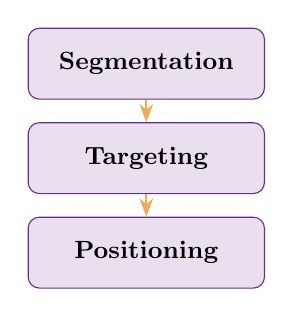
\begin{tikzpicture}[
        stp/.style={draw=cuhkpurple, fill=cuhkpurple!15, rounded corners,
                      minimum width=3cm, minimum height=0.9cm,
                      font=\small\bfseries}
      ]
        \node[stp] (s) at (0,3) {Segmentation};
        \node[stp] (t) at (0,1.8) {Targeting};
        \node[stp] (p) at (0,0.6) {Positioning};

        \draw[-{Stealth}, thick, cuhkgold] (s) -- (t);
        \draw[-{Stealth}, thick, cuhkgold] (t) -- (p);
      \end{tikzpicture}
    \end{column}
  \end{columns}

  \vspace{0.3em}
  {\small \textcolor{cuhkpurple}{$\rightarrow$ Marketing decisions at each
    stage require \textbf{information}. How do we get it systematically?}}
  \source{Lam (2023), pp.3--4}
\end{frame}

% ======================================================================
% ACT 2: WHAT IS MARKETING RESEARCH?
% ======================================================================

\begin{frame}{}
  \begin{center}
    {\Large\textcolor{cuhkpurple}{\textbf{Part II}}}\\[0.5em]
    {\LARGE\textbf{What is Marketing Research?}}\\[1em]
    {\normalsize Malhotra (2020), Chapter 1 \& Lam (2023), Chapter 2}
  \end{center}
\end{frame}

% ------------------------------------------------------------------
\begin{frame}{Defining Marketing Research}
  \begin{block}{Malhotra's Definition}
    \highlight{Marketing research} is the \textbf{systematic} and
    \textbf{objective} \textcolor{cuhkpurple}{identification, collection,
    analysis, dissemination, and use of information} for the purpose of
    improving \textcolor{cuhkpurple}{decision making} related to the
    identification and solution of \textcolor{cuhkpurple}{problems and
    opportunities} in marketing.
  \end{block}
  \source{Malhotra (2020), p.32}
\end{frame}

% ------------------------------------------------------------------
\begin{frame}{Breaking Down the Definition}
  \begin{columns}
    \begin{column}{0.48\textwidth}
      \begin{block}{Systematic}
        \begin{itemize}
          \item Plan each stage
          \item Follow the procedure
          \item Use the scientific method
        \end{itemize}
      \end{block}
    \end{column}
    \begin{column}{0.48\textwidth}
      \begin{block}{Objective}
        \begin{itemize}
          \item Accurate
          \item Free of bias
          \item Impartial analysis
        \end{itemize}
      \end{block}
    \end{column}
  \end{columns}

  \vspace{1em}
  \begin{exampleblock}{Purpose}
    Improving \textbf{decision making} related to the identification and
    solution of \textbf{problems and opportunities} in marketing.
  \end{exampleblock}
  \source{Malhotra (2020), p.32}
\end{frame}

% ------------------------------------------------------------------
\begin{frame}{AMA Definition of Marketing Research}
  \begin{block}{American Marketing Association (2023)}
    ``Marketing research is the function that \textbf{links the consumer,
    customer and public to the marketer through information} ---
    information used to identify and define opportunities and problems;
    generate, refine, and evaluate actions; monitor performance; and
    improve understanding of it as a process.''
  \end{block}

  \vspace{0.5em}
  It specifies the information required, designs the method for collecting
  information, manages and implements the data collection process, analyzes
  the results, and communicates the findings and their implications.

  \source{AMA (2023); Lam (2023), p.7}
\end{frame}

% ------------------------------------------------------------------
\begin{frame}{Classification of Marketing Research}
  \begin{center}
    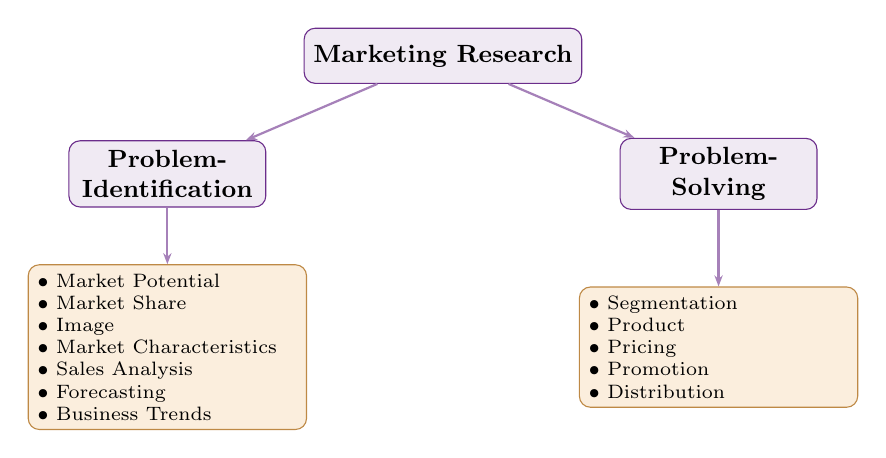
\begin{tikzpicture}[
      box/.style={draw=cuhkpurple, fill=cuhkpurple!10, rounded corners,
                   minimum width=2.5cm, minimum height=0.7cm,
                   font=\small\bfseries, align=center},
      leaf/.style={draw=cuhkgold!80!black, fill=cuhkgold!20,
                    rounded corners, minimum width=3.5cm,
                    font=\scriptsize, align=left, text width=3.3cm},
      arr/.style={-{Stealth[length=4pt]}, thick, cuhkpurple!60}
    ]
      \node[box] (mr) at (0,3.5) {Marketing Research};
      \node[box] (pi) at (-3.5,2) {Problem-\\Identification};
      \node[box] (ps) at (3.5,2) {Problem-\\Solving};

      \draw[arr] (mr) -- (pi);
      \draw[arr] (mr) -- (ps);

      \node[leaf] (pi_list) at (-3.5,-0.2) {
        $\bullet$ Market Potential\\
        $\bullet$ Market Share\\
        $\bullet$ Image\\
        $\bullet$ Market Characteristics\\
        $\bullet$ Sales Analysis\\
        $\bullet$ Forecasting\\
        $\bullet$ Business Trends
      };
      \draw[arr] (pi) -- (pi_list);

      \node[leaf] (ps_list) at (3.5,-0.2) {
        $\bullet$ Segmentation\\
        $\bullet$ Product\\
        $\bullet$ Pricing\\
        $\bullet$ Promotion\\
        $\bullet$ Distribution
      };
      \draw[arr] (ps) -- (ps_list);
    \end{tikzpicture}
  \end{center}
  \source{Malhotra (2020), p.33}
\end{frame}

% ------------------------------------------------------------------
\begin{frame}{Problem-Solving Research in Detail}
  \begin{description}
    \item[\textcolor{cuhkpurple}{Segmentation}]
      Number of segments, size, demographics, lifestyle, media habits
    \item[\textcolor{cuhkpurple}{Product}]
      Test concept, optimal design, package, positioning
    \item[\textcolor{cuhkpurple}{Price}]
      Price elasticity, impact on brand selection, product line pricing
    \item[\textcolor{cuhkpurple}{Promotion}]
      Sales--promotion relationship, copy/media decisions, ad effectiveness
    \item[\textcolor{cuhkpurple}{Distribution}]
      Retail coverage, category--channel preference
  \end{description}
  \source{Malhotra (2020), p.33}
\end{frame}

% ------------------------------------------------------------------
\begin{frame}{Role of MR in Decision-Making}
  \begin{columns}
    \begin{column}{0.35\textwidth}
      \begin{block}{AMA}
        ``Marketing research \ldots{} links the consumer, customer, and
        public to the marketer through \textbf{information}.''
      \end{block}
      \source{Malhotra (2020), p.37}
    \end{column}
    \begin{column}{0.6\textwidth}
      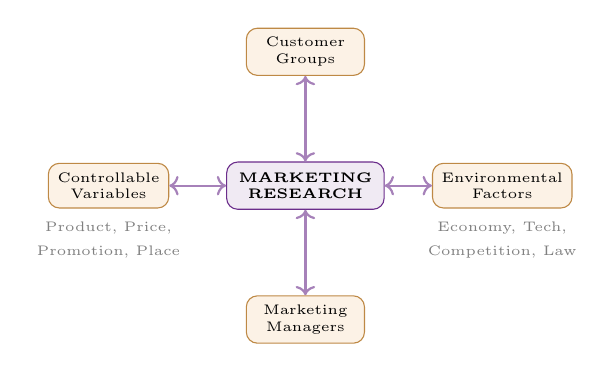
\begin{tikzpicture}[
        box/.style={draw=cuhkpurple, fill=cuhkpurple!10, rounded corners,
                     minimum width=2cm, minimum height=0.6cm,
                     font=\tiny\bfseries, align=center},
        smallbox/.style={draw=cuhkgold!80!black, fill=cuhkgold!15,
                          rounded corners, font=\tiny, align=center,
                          minimum width=1.5cm, minimum height=0.5cm},
        arr/.style={-{Stealth[length=3pt]}, cuhkpurple!60, thick}
      ]
        \node[box] (mr) at (3,2.5) {MARKETING\\RESEARCH};
        \node[smallbox] (cv) at (0.5,2.5) {Controllable\\Variables};
        \node[smallbox] (ef) at (5.5,2.5) {Environmental\\Factors};
        \node[smallbox] (cg) at (3,4.2) {Customer\\Groups};
        \node[smallbox] (mm) at (3,0.8) {Marketing\\Managers};

        \draw[arr, <->] (cv) -- (mr);
        \draw[arr, <->] (ef) -- (mr);
        \draw[arr, <->] (cg) -- (mr);
        \draw[arr, <->] (mm) -- (mr);

        \node[font=\tiny, text=gray, below=0.05cm of cv] {Product, Price,};
        \node[font=\tiny, text=gray, below=0.35cm of cv] {Promotion, Place};
        \node[font=\tiny, text=gray, below=0.05cm of ef] {Economy, Tech,};
        \node[font=\tiny, text=gray, below=0.35cm of ef] {Competition, Law};
      \end{tikzpicture}
    \end{column}
  \end{columns}
\end{frame}

% ------------------------------------------------------------------
\begin{frame}{Exercise: Marketing Research in Practice}
  In the following 6 examples of marketing research:
  \begin{itemize}
    \item What \textbf{information} does the firm collect?
    \item \textbf{How} did the firm collect the information?
    \item What \textbf{decision(s)} did MR lead to?
  \end{itemize}

  \vspace{0.5em}
  {\small
  \begin{tabular}{llll}
    \toprule
    \textbf{Firm} & \textbf{Information} & \textbf{Approach} &
      \textbf{Decision} \\
    \midrule
    Starbucks & & & \\
    Apple & & & \\
    McDonald's & & & \\
    LEGO & & & \\
    Dove & & & \\
    Zappos & & & \\
    \bottomrule
  \end{tabular}
  }

  \vspace{0.5em}
  {\small\textcolor{cuhkpurple}{Discuss with your neighbor (3 minutes).}}
\end{frame}

% ------------------------------------------------------------------
\begin{frame}{When NOT to Conduct Marketing Research}
  Information is not free. MR may \textbf{not} be a good idea if\ldots

  \vspace{0.5em}
  \begin{itemize}
    \item The \textbf{cost of information outweighs its benefit}
      \begin{itemize}
        \item Information is already available
        \item Decisions are already made
      \end{itemize}
    \item \textbf{Resource constraints} (for conducting research and
          implementing findings)
    \item \textbf{Management's attitude} (not willing to act on findings)
  \end{itemize}

  \vspace{1em}
  \begin{columns}
    \begin{column}{0.48\textwidth}
      \begin{exampleblock}{MR Can}
        \begin{itemize}
          \item Identify opportunities and threats
          \item Gain consumer insights
          \item Evaluate strategies
        \end{itemize}
      \end{exampleblock}
    \end{column}
    \begin{column}{0.48\textwidth}
      \begin{alertblock}{MR Cannot}
        \begin{itemize}
          \item Predict the future with certainty
          \item Solve all problems
          \item Provide instant results
        \end{itemize}
      \end{alertblock}
    \end{column}
  \end{columns}
\end{frame}

% ======================================================================
% ACT 3: THE MARKETING RESEARCH PROCESS
% ======================================================================

\begin{frame}{}
  \begin{center}
    {\Large\textcolor{cuhkpurple}{\textbf{Part III}}}\\[0.5em]
    {\LARGE\textbf{The Marketing Research Process}}\\[1em]
    {\normalsize Malhotra (2020), Chapter 2}
  \end{center}
\end{frame}

% ------------------------------------------------------------------
\begin{frame}{The 6-Step Marketing Research Process}
  \begin{center}
    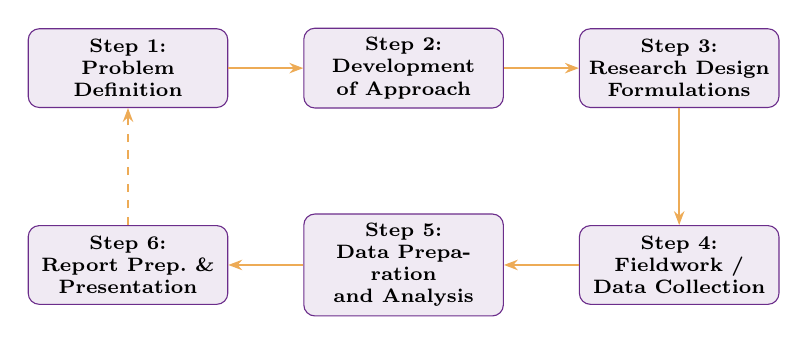
\begin{tikzpicture}[
      stepbox/.style={draw=cuhkpurple, fill=cuhkpurple!10, rounded corners,
                    minimum width=2.5cm, minimum height=1cm,
                    font=\scriptsize\bfseries, align=center,
                    text width=2.3cm},
      arr/.style={-{Stealth[length=5pt]}, thick, cuhkgold}
    ]
      \node[stepbox] (s1) at (0,0) {Step 1:\\Problem\\Definition};
      \node[stepbox] (s2) at (3.5,0) {Step 2:\\Development\\of Approach};
      \node[stepbox] (s3) at (7,0) {Step 3:\\Research Design\\Formulations};
      \node[stepbox] (s4) at (7,-2.5) {Step 4:\\Fieldwork /\\Data Collection};
      \node[stepbox] (s5) at (3.5,-2.5) {Step 5:\\Data Preparation\\and Analysis};
      \node[stepbox] (s6) at (0,-2.5) {Step 6:\\Report Prep.~\&\\Presentation};

      \draw[arr] (s1) -- (s2);
      \draw[arr] (s2) -- (s3);
      \draw[arr] (s3) -- (s4);
      \draw[arr] (s4) -- (s5);
      \draw[arr] (s5) -- (s6);
      \draw[arr, dashed] (s6) -- (s1);
    \end{tikzpicture}
  \end{center}
  \source{Malhotra (2020), p.32}
\end{frame}

% ------------------------------------------------------------------
\begin{frame}{Step 1: Problem Definition}
  The \textbf{most important} step --- a problem well defined is half solved.

  \vspace{0.5em}
  \begin{block}{Two Types of Problems}
    \begin{description}
      \item[\textcolor{cuhkpurple}{Management Decision Problem}]
        What should the decision maker do?\\
        {\small E.g., ``Should McDonald's change its menu?''}
      \item[\textcolor{cuhkpurple}{Marketing Research Problem}]
        What information is needed and how should it be obtained?\\
        {\small E.g., ``Determine consumer preferences for menu items and
        competitive positioning.''}
    \end{description}
  \end{block}

  \vspace{0.5em}
  {\small The management decision problem is \textbf{action-oriented}.
  The marketing research problem is \textbf{information-oriented}.}
\end{frame}

% ------------------------------------------------------------------
\begin{frame}{Gathering Background Information}
  Before defining the problem, we need to learn about the \textbf{context}.

  \vspace{0.5em}
  \textbf{Sources of information:}
  \begin{itemize}
    \item Decision makers
    \item Industry experts
    \item Secondary data
    \item Qualitative research
  \end{itemize}

  \vspace{0.5em}
  \begin{block}{7 Types of Information (PROBLEM)}
    \textbf{P}ast Information and Forecasts,
    \textbf{R}esources and Constraints,
    \textbf{O}bjectives,
    \textbf{B}uyer Behavior,
    \textbf{L}egal Environment,
    \textbf{E}conomic Environment,
    \textbf{M}arketing and Technological Skills
  \end{block}
  \source{Malhotra (2020), Ch.2}
\end{frame}

% ------------------------------------------------------------------
\begin{frame}{Talking to the Decision Maker}
  Talking to the decision maker (DM) is
  \textcolor{cuhkpurple}{\textbf{extremely important}}.

  \vspace{0.5em}
  Use the \textbf{problem audit} framework:
  \begin{itemize}
    \item \textbf{Events} that led to the research\\
      {\small\textcolor{gray}{E.g., KFC launched new products; McDonald's
      campaign not performing well}}
    \item \textbf{Alternatives} available\\
      {\small\textcolor{gray}{Add new items, cut price, change advertising}}
    \item \textbf{Criteria} for evaluating alternatives\\
      {\small\textcolor{gray}{Market share, profits, sales volume}}
    \item \textbf{Information} needed\\
      {\small\textcolor{gray}{Marketing mix data on McDonald's and competitors}}
    \item \textbf{Corporate culture}\\
      {\small\textcolor{gray}{How strategic decisions are made and influenced}}
  \end{itemize}

  \vspace{0.3em}
  {\small\textbf{Challenge:} Access to DM may be difficult (hierarchy,
  multiple decision makers).}
  \source{Malhotra (2020), Ch.2}
\end{frame}

% ------------------------------------------------------------------
\begin{frame}{Step 2: Developing an Approach}
  \begin{center}
    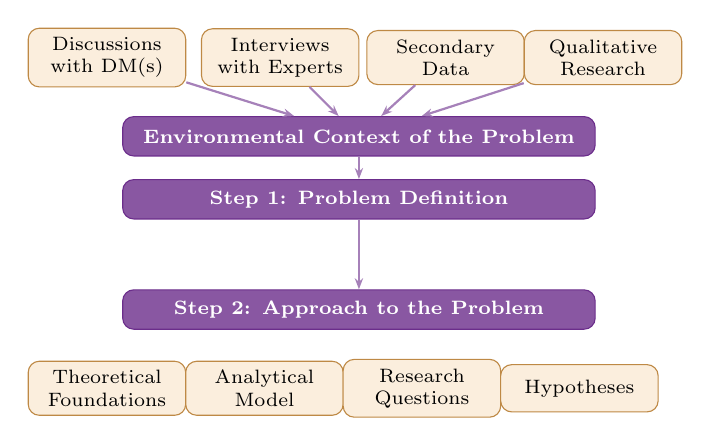
\begin{tikzpicture}[
      task/.style={draw=cuhkgold!80!black, fill=cuhkgold!20,
                    rounded corners, font=\scriptsize, align=center,
                    minimum width=2cm, minimum height=0.6cm},
      stage/.style={draw=cuhkpurple, fill=cuhkpurple!80, text=white,
                     rounded corners, font=\scriptsize\bfseries,
                     align=center, minimum width=6cm, minimum height=0.5cm},
      comp/.style={draw=cuhkgold!80!black, fill=cuhkgold!20,
                    rounded corners, font=\scriptsize, align=center,
                    minimum width=2cm, minimum height=0.6cm},
      arr/.style={-{Stealth[length=4pt]}, thick, cuhkpurple!60}
    ]
      \node[task] (t1) at (-2.5,4) {Discussions\\with DM(s)};
      \node[task] (t2) at (-0.3,4) {Interviews\\with Experts};
      \node[task] (t3) at (1.8,4) {Secondary\\Data};
      \node[task] (t4) at (3.8,4) {Qualitative\\Research};

      \node[stage] (env) at (0.7,3) {Environmental Context of the Problem};
      \node[stage] (pd) at (0.7,2.2) {Step 1: Problem Definition};
      \node[stage] (ap) at (0.7,0.8) {Step 2: Approach to the Problem};

      \draw[arr] (t1) -- (env);
      \draw[arr] (t2) -- (env);
      \draw[arr] (t3) -- (env);
      \draw[arr] (t4) -- (env);
      \draw[arr] (env) -- (pd);
      \draw[arr] (pd) -- (ap);

      \node[comp] at (-2.5,-0.2) {Theoretical\\Foundations};
      \node[comp] at (-0.5,-0.2) {Analytical\\Model};
      \node[comp] at (1.5,-0.2) {Research\\Questions};
      \node[comp] at (3.5,-0.2) {Hypotheses};
    \end{tikzpicture}
  \end{center}
  \source{Malhotra (2020), p.61}
\end{frame}

% ------------------------------------------------------------------
\begin{frame}{Steps 3--6: Overview}
  \begin{description}
    \item[\textcolor{cuhkpurple}{Step 3: Research Design Formulations}]
      Type of research (exploratory, descriptive, causal), measurement and
      scaling, questionnaire design, sampling process
    \item[\textcolor{cuhkpurple}{Step 4: Fieldwork / Data Collection}]
      Selection, training, and supervision of field workers; data
      collection methods (surveys, observations, experiments)
    \item[\textcolor{cuhkpurple}{Step 5: Data Preparation and Analysis}]
      Editing, coding, transcribing; statistical analysis
      ($\chi^2$, $t$-test, ANOVA, regression)
    \item[\textcolor{cuhkpurple}{Step 6: Report Preparation \& Presentation}]
      Document findings, conclusions, and recommendations; present to
      management
  \end{description}

  \vspace{0.5em}
  \textcolor{cuhkpurple}{$\rightarrow$ We will cover each step in detail
  across this course.}
\end{frame}

% ------------------------------------------------------------------
\begin{frame}{Course Roadmap: MR Process $\times$ Lectures}
  \begin{center}
    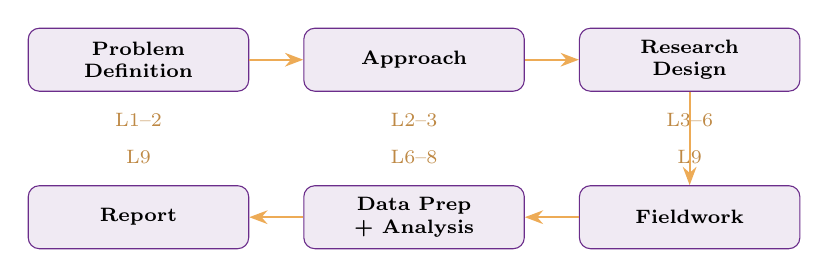
\begin{tikzpicture}[
      stepbox/.style={draw=cuhkpurple, fill=cuhkpurple!10, rounded corners,
                    minimum width=2.8cm, minimum height=0.8cm,
                    font=\scriptsize\bfseries, align=center},
      lec/.style={font=\scriptsize, text=cuhkgold!80!black}
    ]
      \node[stepbox] (s1) at (0,2) {Problem\\Definition};
      \node[stepbox] (s2) at (3.5,2) {Approach};
      \node[stepbox] (s3) at (7,2) {Research\\Design};
      \node[stepbox] (s4) at (7,0) {Fieldwork};
      \node[stepbox] (s5) at (3.5,0) {Data Prep\\+ Analysis};
      \node[stepbox] (s6) at (0,0) {Report};

      \node[lec, below=0.15cm] at (s1.south) {L1--2};
      \node[lec, below=0.15cm] at (s2.south) {L2--3};
      \node[lec, below=0.15cm] at (s3.south) {L3--6};
      \node[lec, above=0.15cm] at (s4.north) {L9};
      \node[lec, above=0.15cm] at (s5.north) {L6--8};
      \node[lec, above=0.15cm] at (s6.north) {L9};

      \draw[-{Stealth}, thick, cuhkgold] (s1) -- (s2);
      \draw[-{Stealth}, thick, cuhkgold] (s2) -- (s3);
      \draw[-{Stealth}, thick, cuhkgold] (s3) -- (s4);
      \draw[-{Stealth}, thick, cuhkgold] (s4) -- (s5);
      \draw[-{Stealth}, thick, cuhkgold] (s5) -- (s6);
    \end{tikzpicture}
  \end{center}

  \vspace{0.5em}
  {\small Additional: L10 covers \textbf{Experimentation} (causal design)
  and \textbf{Market Sizing}.}
\end{frame}

% ======================================================================
% ACT 4: MARKETING RESEARCH OR NOT?
% ======================================================================

\begin{frame}{}
  \begin{center}
    {\Large\textcolor{cuhkpurple}{\textbf{Part IV}}}\\[0.5em]
    {\LARGE\textbf{Marketing Research or Not?}}\\[1em]
    {\normalsize Lam (2023), Chapter 2}
  \end{center}
\end{frame}

% ------------------------------------------------------------------
\begin{frame}{Not All Decisions Need MR}
  \begin{exampleblock}{Example: The Bus Coin Problem}
    A bus company needs to count coins collected from passengers.
    Should we research how to build a better coin-sorting machine?
  \end{exampleblock}

  \vspace{0.5em}
  \textbf{Reframe the problem:} The real need is a \textbf{payment mechanism}
  that lets each traveler pay quickly and easily.

  \vspace{0.5em}
  Solutions that don't require MR:
  \begin{itemize}
    \item Stored-value travel cards (Octopus)
    \item QR code payments from mobile phones
  \end{itemize}

  \vspace{0.5em}
  \textcolor{cuhkpurple}{\textbf{Lesson:} Define the right problem before
  deciding whether you need research.}
  \source{Lam (2023), p.8}
\end{frame}

% ------------------------------------------------------------------
\begin{frame}{Example: Shampoo Promotion (Solving Without MR)}
  \textbf{Problem:} A retailer wants an appealing gift for shampoo purchases
  (HK\$25/bottle). Marketing budget constraint: the gift cannot exceed 20\%
  of retail price (HK\$5).

  \vspace{0.5em}
  \begin{block}{Creative Solution Using the 6Cs}
    Instead of conducting MR on gift preferences:
    \begin{enumerate}
      \item Find a \textbf{collaborator} (quick service restaurant)
      \item Offer HK\$5 cash coupon with each shampoo bottle
      \item Negotiate discount: pay only HK\$4 per redeemed coupon
      \item At 25\% redemption $\rightarrow$ cost = HK\$4 / (4 $\times$
            HK\$25) = \textbf{4\%} of sales
    \end{enumerate}
  \end{block}

  \vspace{0.3em}
  {\small\textcolor{cuhkpurple}{$\rightarrow$ Analytical thinking solved the
  problem without any market research.}}
  \source{Lam (2023), pp.8--9}
\end{frame}

% ------------------------------------------------------------------
\begin{frame}[fragile]{Example: Chocolate Bar Upsize (Breakeven Analysis)}
  \textbf{Should we offer 15\% more chocolate for the same price (HK\$70)?}

  \vspace{0.3em}
  \begin{columns}
    \begin{column}{0.55\textwidth}
      Given: Variable cost of 200\,g = HK\$20.

      New cost for 230\,g = HK\$20 $\times$ $\frac{230}{200}$ = HK\$23

      \vspace{0.3em}
      \textbf{Breakeven:}
      \begin{align*}
        S \times (\$70 - \$20) &= B \times (\$70 - \$23) \\
        S \times \$50 &= B \times \$47 \\
        \frac{B}{S} &= \frac{\$50}{\$47} = 1.06
      \end{align*}
    \end{column}
    \begin{column}{0.4\textwidth}
      \begin{alertblock}{Result}
        Need only \textbf{6\% increase} in units sold to maintain the same
        profit.
      \end{alertblock}
      \vspace{0.3em}
      If current market share = 35\%:\\
      New share $\approx$ \textbf{42.7\%}\\
      (assuming market size constant)
    \end{column}
  \end{columns}

  \vspace{0.3em}
  {\small\textcolor{cuhkpurple}{$\rightarrow$ Financial analysis can answer
  the question --- no MR needed.}}
  \source{Lam (2023), pp.9--11}
\end{frame}

% ------------------------------------------------------------------
\begin{frame}{Key Takeaway: Think Before You Research}
  \begin{center}
    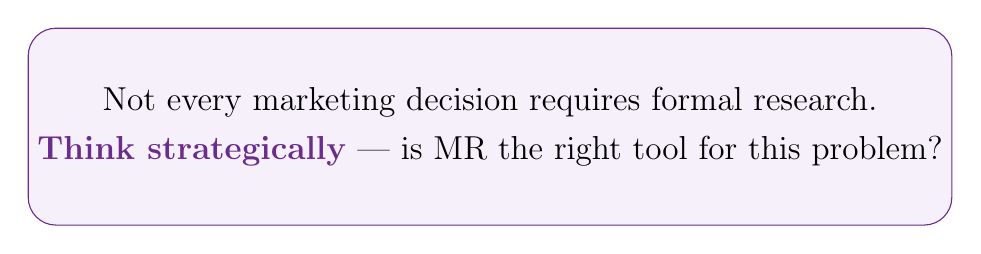
\begin{tikzpicture}
      \node[draw=cuhkpurple, fill=lightbg, rounded corners=10pt,
            minimum width=10cm, minimum height=2.5cm, align=center,
            font=\large] {
        Not every marketing decision requires formal research.\\[0.3em]
        \textcolor{cuhkpurple}{\textbf{Think strategically}} ---
        is MR the right tool for this problem?
      };
    \end{tikzpicture}
  \end{center}

  \vspace{0.5em}
  Ask yourself:
  \begin{enumerate}
    \item Can I \textbf{reframe} the problem? (bus coin example)
    \item Can I solve it with \textbf{creative thinking} and the 6Cs?
          (shampoo promotion)
    \item Can I use \textbf{existing data} and financial analysis?
          (chocolate upsize)
    \item Only then: design and conduct marketing research
  \end{enumerate}
\end{frame}

% ======================================================================
% ACT 5: R LAB — GETTING STARTED
% ======================================================================

\begin{frame}{}
  \begin{center}
    {\Large\textcolor{cuhkpurple}{\textbf{Part V}}}\\[0.5em]
    {\LARGE\textbf{R Lab: Getting Started}}\\[1em]
    {\normalsize Lam (2023), Appendix 4, Sections 1--5}
  \end{center}
\end{frame}

% ------------------------------------------------------------------
\begin{frame}{Why R?}
  \begin{columns}
    \begin{column}{0.55\textwidth}
      \begin{itemize}
        \item \textbf{Free} and open-source
        \item Runs on Windows, macOS, Linux
        \item Powerful for statistical analysis and visualization
        \item Used in academia \emph{and} industry
        \item No license needed --- use it on your own computer, anytime
      \end{itemize}

      \vspace{0.5em}
      In this course, we will learn R progressively:
      \begin{itemize}
        \item Today: Installation + basics
        \item Over 10 lectures: from arithmetic to regression, NLP, and
              graphics
      \end{itemize}
    \end{column}
    \begin{column}{0.4\textwidth}
      \begin{block}{R in this Course}
        \begin{tabular}{ll}
          \toprule
          \textbf{L\#} & \textbf{R Topic} \\
          \midrule
          1 & Install, Console \\
          2 & Arithmetic, Functions \\
          3 & Conditions, Loops \\
          4 & Read/Write Files \\
          6 & $\chi^2$, $r$, $t$-test \\
          7 & ANOVA \\
          8 & Regression \\
          9 & NLP, Web Scraping \\
          10 & Graphics \\
          \bottomrule
        \end{tabular}
      \end{block}
    \end{column}
  \end{columns}
  \source{Lam (2023), p.141}
\end{frame}

% ------------------------------------------------------------------
\begin{frame}[fragile]{Installing R}
  \begin{enumerate}
    \item Go to \textcolor{cuhkpurple}{\texttt{https://www.r-project.org}}
    \item Click ``Getting Started'' $\rightarrow$ ``Download R''
    \item Choose your operating system (Windows / macOS / Linux)
    \item Follow the installation steps
  \end{enumerate}

  \vspace{0.5em}
  After installation, open the \textbf{R Console}:

  \begin{lstlisting}
> # The > symbol is the R prompt
> # R is ready for your commands!
  \end{lstlisting}

  \vspace{0.3em}
  {\small The \rcode{>} prompt means R is ready to take your command.
  You can press the \textbf{up arrow} to recall previous commands.}
  \source{Lam (2023), pp.141--143}
\end{frame}

% ------------------------------------------------------------------
\begin{frame}[fragile]{R Console Basics}
  \begin{lstlisting}
# Say hello to the world
print("Hello World")
[1] "Hello World"

# Get help on a function
help(mean)

# Check and set working directory
getwd()
[1] "/Users/yourname"
setwd("/Users/yourname/Documents/R-folder")
  \end{lstlisting}

  \vspace{0.3em}
  {\small\textbf{Tip:} The \rcode{[1]} tells you this is the first element
  in the output.}
  \source{Lam (2023), pp.142--144}
\end{frame}

% ------------------------------------------------------------------
\begin{frame}[fragile]{R as a Calculator}
  \begin{columns}
    \begin{column}{0.48\textwidth}
      \begin{lstlisting}
# Basic arithmetic
8 + 2      # [1] 10
8 - 2      # [1] 6
8 * 2      # [1] 16
8 / 2      # [1] 4
8 ^ 2      # [1] 64
16 ^ 0.5   # [1] 4
      \end{lstlisting}
    \end{column}
    \begin{column}{0.48\textwidth}
      \begin{lstlisting}
# Operator precedence
8 + 2 * 3  # [1] 14
(8 + 2) * 3  # [1] 30

# Use print() in RStudio
print(8 + 2)  # [1] 10
print((8 + 2) * 3)  # [1] 30
      \end{lstlisting}
    \end{column}
  \end{columns}

  \vspace{0.5em}
  \begin{alertblock}{Important}
    In the R Console, results are displayed automatically.
    In \textbf{RStudio}, use \rcode{print()} to see output explicitly.
  \end{alertblock}
  \source{Lam (2023), pp.143, 146--147}
\end{frame}

% ------------------------------------------------------------------
\begin{frame}{Installing and Using RStudio}
  RStudio provides a more convenient environment for writing R programs.

  \vspace{0.5em}
  \begin{enumerate}
    \item \textbf{Install R first} (from r-project.org)
    \item Download RStudio from
          \textcolor{cuhkpurple}{\texttt{https://posit.co/}}
    \item Open RStudio $\rightarrow$ File $\rightarrow$ Open Project
  \end{enumerate}

  \vspace{0.5em}
  \begin{block}{RStudio Advantages}
    \begin{itemize}
      \item Create, read, modify, and execute R scripts (\texttt{.R} files)
      \item Organize code and data in projects
      \item View plots, help, and environment in one window
    \end{itemize}
  \end{block}

  \vspace{0.3em}
  {\small\textbf{In-class:} Install both R and RStudio on your laptop now.
  We will use RStudio for all R labs going forward.}
  \source{Lam (2023), pp.144--145}
\end{frame}

% ------------------------------------------------------------------
\begin{frame}[fragile]{Variables and Assignment}
  \begin{lstlisting}
# Assignment uses <- (less-than + hyphen)
x <- 1
y <- 2
print(x + y)
[1] 3

# R is case-sensitive!
X <- 1    # uppercase X = 1
x <- 2    # lowercase x = 2

# Comments start with #
L <- 7   # Length of a rectangle
W <- 2   # Width of a rectangle
print(L * W)  # Area
[1] 14
  \end{lstlisting}
  \source{Lam (2023), pp.145, 147--148}
\end{frame}

% ======================================================================
% SUMMARY & NEXT TIME
% ======================================================================

\begin{frame}{Summary}
  \begin{enumerate}
    \item \textbf{Marketing} is about creating and exchanging value
          (AMA definition, 5/6Cs, STP)
    \item \textbf{Marketing research} is the systematic and objective
          process of gathering information for decision-making
    \item Two types: \textbf{problem-identification} and
          \textbf{problem-solving} research
    \item The \textbf{6-step MR process} begins with problem definition
    \item Not every decision requires MR ---
          \textbf{think strategically first}
    \item \textbf{R and RStudio} are our tools for data analysis
          throughout this course
  \end{enumerate}

  \vspace{0.5em}
  \begin{block}{Readings for Next Time}
    \begin{itemize}
      \item Iansiti et al.\ (2016), \emph{Product Development Fundamentals}
      \item Lam (2023), Chapter 3
    \end{itemize}
  \end{block}
\end{frame}

% ------------------------------------------------------------------
\begin{frame}{}
  \begin{center}
    {\LARGE\textcolor{cuhkpurple}{\textbf{Thank You}}}\\[1em]
    {\large Questions?}\\[2em]
    {\normalsize\textcolor{gray}{MKTG5012 Marketing Research}}\\
    {\normalsize\textcolor{gray}{CUHK Business School}}
  \end{center}
\end{frame}

\end{document}
